\chapter{Preliminaries}
\label{ch:preliminaries}

\section{Reinforcement Learning}
\label{sec:preliminaries:rl}

In reinforcement learning (RL) an agent that interacts with an environment is trained to maximize a reward function. The agent takes actions based on observations from the environment. The problem is often formulated as a Markov decision process (MDP). The notation in the following sections is taken from OpenAI Spinning Up \cite{WelcomeSpinningDeep}.

\subsection{Markov Decision Process}
\label{sec:preliminaries:rl:mdp}
\begin{definition}
    \label{def:mdp}
    Given a
    \begin{itemize}
        \item Set of states \emph{S}
        \item Set of actions \emph{A}
        \item Transition probability function $\emph{P}:S\times A\times S \rightarrow [0,1]$
        \item Reward function $\emph{R}: S\times A\times S \rightarrow [0,1]$
        \item Start state distribution $\rho_0$
        \item Discount factor $\gamma$
    \end{itemize}
    the tuple $(S, A, P, R, \rho_0, \gamma)$ is called a Markov decision process (MDP).
\end{definition}
A trajectory $\tau$ is a sequence of states and actions $\tau = (s_0, a_0, s_1, a_1, \dots)$. At a discrete time step $t$, the transition function $P(s'|s,a)=P(s_{t+1}=s'|s_t=s, a_t=s)$ is given by the probability of reaching state $s_{t+1}$ if the current state is $s_t$ and action $a_t$ is taken. According to the Markov property the next state $s_{t+1}$ only depends on the current state $s_t$ and action $a_t$.

The reward function $r_t = R(s_t, a_t, s_{t+1})$ describes the reward for a state-action-next-state triplet. $R$ also denotes the return of a trajectory, given by the discounted sum of rewards:
\begin{equation}
    R(\tau) = \sum^\infty_{t=0} \gamma^t r_t
    \label{eq:trajectory-return}
\end{equation}
The discount factor $\gamma$ describes how import rewards in the future are in contrast to immediate rewards.

Most of the agents in this work do not use the states of the environment as observations, but an image of the environment. In this case the MDP is considered to be partially observable, as not all state information might be observable at every time step.


\subsubsection{Constrained Markov Decision Process}
\label{sec:preliminaries:rl:cmdp}

Multiple definitions of constrained Markov decision processes (CMDP) exist. In this work a CMDP is a MDP extended with a cost function $C:S\times A\times S \rightarrow [0,1]$ and a threshold $\delta \in \mathbb{R}_{\geq 0}$.
Similar to the reward in equation \ref{eq:trajectory-return}, this can be extended for a trajectory:
\begin{equation}
    C(\tau) = \sum^\infty_{t=0} \gamma^t c_t
    \label{eq:trajectory-cost}
\end{equation}
with $c_t = C(s_t,a_t,c_{t+1})$ denoting the cost of a state-action-next-state triplet in a trajectory $\tau = (s_0, a_0, s_1, a_1, \dots)$.
If $C(\tau) \leq \delta$ the trajectory $\tau$ fulfills the constraint.

\subsection{The Reinforcement Learning Goal}
\label{sec:preliminaries:rl:rl-goal}

The agent selects which action to take in the environment based on a policy $\pi$. RL aims to find the policy that maximizes the expected reward. Only stochastic policies $\pi(a|s)$ are used in this work. For a state $s_t$, an action $a_t$ can be sampled from the policy: $a_t \sim \pi(\cdot|s_t)$. In the following, if the state is evident from the context, this will be written as $a\sim\pi$. When combined with the transition probability function, it is also possible to sample whole trajectories $\tau\sim\pi$.

Given the transition probability function $P$, the reward function $R$, and a policy $\pi$, the probability of a trajectory $\tau$ of length $T$ can be written as:
\begin{equation}
    P(\tau|\pi) = \rho_0(s_0)\prod^{T-1}_{t=0}P(s_{t+1}|s_t,a_t)\pi(a_t|s_t)
\end{equation}
The expected return $J_R(\pi)$ when using the policy $\pi$ can then be written as:
\begin{equation}
    J_R(\pi) = \int_\tau P(\tau|\pi)R(\tau) = \underset{\tau \sim \pi}{\mathbb{E}} [R(\tau)]
    \label{eq:trajectory-expected-return}
\end{equation}
The goal of RL, finding the optimal policy $\pi^*$ that maximizes the expected reward, can then be denoted as:
\begin{equation}
    \pi^* = \underset{\pi}{\arg\max} ~J_R(\pi)
    \label{eq:optimal-policy-simple}
\end{equation}
Combining equations \ref{eq:trajectory-return}, \ref{eq:trajectory-expected-return}, and \ref{eq:optimal-policy-simple} yields:
\begin{equation}
    \pi^* = \underset{\pi}{\arg\max} \underset{\tau\sim\pi}{\mathbb{E}}\Big[\sum^\infty_{t=0}\gamma^t R(s_t,a_t,s_{t+1})\Big]
    \label{eq:optimal-policy}
\end{equation}
For a CMDP the expected cost when using policy $\pi$ can be written as:
\begin{equation}
    J_C(\pi) = \int_\tau P(\tau|\pi)C(\tau) = \underset{\tau \sim \pi}{\mathbb{E}} [C(\tau)]
\end{equation}
This changes the RL goal for a CMDP to:
\begin{equation}
    \pi^* = \underset{\pi}{\arg\max} ~J_R(\pi),~ s.t.~ J_C(\pi) \leq \delta
\end{equation}

\subsection{Value Functions}
\label{sec:preliminaries:rl:valueFunctions}

The value of a state $s$ or a state-action pair $(s, a)$ under policy $\pi$ can be represented as the expected return when starting in $s$ and following policy $\pi$. In the case of a state-action pair, the initial action is specified as $a$:
\begin{equation}
    V^\pi(s)=\underset{\tau\sim\pi}{\mathbb{E}}[R(\tau)|s_0=s]
\end{equation}
\begin{equation}
    Q^\pi(s,a)=\underset{\tau\sim\pi}{\mathbb{E}}[R(\tau)|s_0=s, a_0=a]
\end{equation}
If all actions are chosen by the optimal policy, the value functions are denoted in the following way:
\begin{equation}
    V^*(s)=\underset{\pi}{\max}\underset{\tau\sim\pi}{\mathbb{E}}[R(\tau)|s_0=s]
\end{equation}
\begin{equation}
    Q^*(s,a)=\underset{\pi}{\max}\underset{\tau\sim\pi}{\mathbb{E}}[R(\tau)|s_0=s, a_0=a]
\end{equation}
Based on the value functions, the Bellman equations can be formulated. They reformulate the value functions as the sum of the reward we expect to get for being in a state $s$ and the expected return from the next state $s'$, discounted by $\gamma$.

%The Bellman equations, which express the value functions as the sum of the reward expected in a state $s$ and the discounted expected return from the next state $s'$, can be derived from the value functions. These equations take the form:

\begin{equation}
    V^\pi(s)=\underset{\begin{subarray}{c}
        a\sim\pi\\
        s'\sim P(\cdot|s,a)
    \end{subarray}}{\mathbb{E}}[R(s,a,s')+\gamma V^\pi(s')]
\end{equation}
\begin{equation}
    Q^\pi(s,a)=\underset{s'\sim P(\cdot|s,a)}{\mathbb{E}}[R(s,a,s')+\gamma \underset{a'\sim\pi}{\mathbb{E}}[Q^\pi(s',a')]]
\end{equation}
Again, when following the optimal policies, this changes to:\begin{equation}
    V^*(s)=\underset{a}{\max}\underset{s'\sim P(\cdot|s,a)}{\mathbb{E}}[R(s,a,s')+\gamma V^*(s')]
\end{equation}
\begin{equation}
    Q^*(s,a)=\underset{s'\sim P(\cdot|s,a)}{\mathbb{E}}[R(s,a,s)+\gamma \underset{a'}{\max}[Q^*(s',a')]]
\end{equation}


\subsection{Soft Actor-Critic}
\label{sec:preliminaries:rl:sac}

Soft Actor-Critic (SAC) \cite{haarnojaOffPolicyMaximumEntropy} is one of the current state of the art RL algorithms. SAC uses entropy regularization to prevent the policy from only learning a single solution to the problem.
\begin{definition}
    Given a random variable $X$, distributed according to $P$, the \emph{entropy} is given by:
    \begin{equation}
        H(P) = \underset{X\sim P}{\mathbb{E}}[-\log P(X)]
    \end{equation}
\end{definition}

The entropy of the policy is used to change the definition of the optimal policy from equation \ref{eq:optimal-policy}, as well as the value functions and bellman equations, to a trade-off between maximizing the return and the entropy of the policy. A parameter $\alpha$ is added to determine the importance of the entropy.
\begin{equation}
    \pi^* = \underset{\pi}{\arg\max} \underset{\tau\sim\pi}{\mathbb{E}}\Big[\sum^\infty_{t=0}\gamma^t \Big(R(s_t,a_t,s_{t+1}) + 
    \alpha H(\pi(\cdot|s_t))\Big)\Big]
    \label{eq:sac-optimal-policy}
\end{equation}
Therefore, also the value functions change:
\begin{equation}
    V^\pi(s)=\underset{\tau\sim\pi}{\mathbb{E}}\Big[\sum^\infty_{t=0}\gamma^t \Big(R(s_t,a_t,s_{t+1}) + 
    \alpha H(\pi(\cdot|s_t))\Big)\Big|s_0=s\Big]
\end{equation}
\begin{equation}
    Q^\pi(s,a)=\underset{\tau\sim\pi}{\mathbb{E}}\Big[\sum^\infty_{t=0}\gamma^t R(s_t,a_t,s_{t+1}) + 
    \alpha \sum^\infty_{t=1}\gamma^t H(\pi(\cdot|s_t))\Big|s_0=s, a_0=a\Big]
\end{equation}
As well as the Bellman equations. However, the state bellman equation is not needed for SAC. It is therefore omitted here.
\begin{align}
    Q^\pi(s,a) &= \underset{s'\sim P(\cdot|s,a)}{\mathbb{E}}\Big[R(s,a,s') + \gamma\underset{a'\sim\pi}{\mathbb{E}}\Big[Q^\pi(s',a') + \alpha H(\pi(\cdot|s'))\Big]\Big]
    \label{eq:sac-bellman-q-1}\\
    &= \underset{\begin{subarray}{c}
        s'\sim P(\cdot|s,a)\\
        a'\sim\pi
    \end{subarray}}{\mathbb{E}}\Big[R(s,a,s') + \gamma\Big(Q^\pi(s',a') + \alpha H(\pi(\cdot|s'))\Big)\Big]
    \label{eq:sac-bellman-q-2}\\
    &= \underset{\begin{subarray}{c}
        s'\sim P(\cdot|s,a)\\
        a'\sim\pi
    \end{subarray}}{\mathbb{E}}\Big[R(s,a,s') + \gamma\Big(Q^\pi(s',a') - \alpha \log\pi(a'|s')\Big)\Big]
    \label{eq:sac-bellman-q-3}
\end{align}
In newer implementations of SAC, $\alpha$ is often learned during training. \cite{haarnojaLearningWalkDeep2019}

SAC is an off-policy method. This means that when executing an action in the environment, the resulting quintuple \emph{state, action, reward, next state, done} $(s,a,r,s',d)$ is not used for training directly, but stored in a replay buffer $D$. The flag $done$ identifies, whether the episode was terminated after this action.

A SAC implementation consists of an actor, i.e. the policy $\pi_\theta$ and a critic, which in turn consists of two Q-functions $Q_{\phi_i}$ $i \in \{1,2\}$. The double-Q trick helps to make the training more robust. All three components are separate neural networks. $\theta$ and $\phi_i$ denote the parameters of the networks. For a training step, a batch of $(s,a,r,s',d)$ transitions is sampled from the replay buffer.

\subsubsection{Training the Critic}
\label{sec:preliminaries:rl:sac-critic}
Since the Q-function as denoted in equation \ref{eq:sac-bellman-q-3} is an expectation, it can be approximated using samples. For a given sample $(s,a,r,s',d)$ from the replay buffer $D$, only the next action $a'$ needs to be sampled from $\pi(\cdot|s')$:
\begin{equation}
    Q^\pi(s,a) \approx r+\gamma(Q^\pi(s',a')-\alpha \log~ \pi(a'|s')),~ a'\sim\pi(\cdot|s')
    \label{eq:q-approx}
\end{equation}
In practice, this is used to create a target to train the Q-functions:
\begin{equation}
    y(r,s',d) = r+\gamma(1-d)\Big(\underset{j=1,2}{\min}Q_{\overline{\phi}_i}(s',a')-\alpha \log~ \pi_\theta(a'|s')\Big),~ a'\sim\pi_\theta(\cdot|s')
    \label{eq:q-target}
\end{equation}
The recursion in the Bellman equation utilizes two Q-functions parameterized with $\overline{\phi}_i$. These are called the target networks and represent older versions of the two Q-functions whose parameters are updated every few training steps with the new parameters $\phi_i$. The use of target networks stabilizes the training. The policy $\pi_\theta$ is used to sample the following action $a'$. The term $1-d$ is necessary since the episode terminated in case of $d=1$, and there is no return from future actions.

With all this in place, the two Q-functions can be trained using gradient descent with:
\begin{equation}
    J_Q(\phi)_i = \underset{(s,a,r,s',d)\sim D}{\mathbb{E}}\Big[\Big(Q_{\phi_i}(s,a)-y(r,s',d)\Big)^2\Big]
    \label{eq:critic-loss}
\end{equation}

\subsubsection{Training the Actor}
\label{sec:preliminaries:rl:sac-actor}

The goal of SAC is to train a policy that is proportional to the exponential of the Q-function. This results in a stochastic policy that, with a high probability, proposes actions whose Q value is also high for a given state.
\begin{definition}
    For two probability distributions \emph{p, q} on the same probability space $X$, the Kullback-Leibler divergence (KL) \cite{kullbackInformationSufficiency1951} is given by:
    \begin{equation}
        D_{KL}(p||q) = \sum_{x\in X}p(x) \log \frac{p(x)}{q(x)}
    \end{equation}
    The KL is a similarity measure between the two distributions. It is always non-negative and zero if and only if  $p = q$. Nevertheless, it is not symmetric.
\end{definition}
The policy parameters can be optimized by minimizing the KL of the policy and the exponential of the Q-function:
\begin{align}
    & \underset{s\sim D}{\mathbb{E}}\Bigg[D_{KL}\Bigg(\pi_\theta(\cdot|s)\Bigg|\Bigg|\frac{\exp\big(\frac{1}{\alpha}Q_\phi(s,\cdot)\big)}{Z_\phi(s)}\Bigg)\Bigg]\\
    &= \underset{s\sim D}{\mathbb{E}}\Bigg[\sum_{a\in A} \pi_\theta(a|s) \log\Bigg(\frac{\pi_\theta(a|s)Z_\phi(s)}{\exp\big(\frac{1}{\alpha}Q_\phi(s,a)\big)}\Bigg)\Bigg]\\
    &= \underset{\begin{subarray}{c}
        s\sim D\\
        a\sim \pi_\theta(\cdot|s)
    \end{subarray}}{\mathbb{E}}\Big[\log\pi_\theta(a|s)+\log Z_\phi(s)-\frac{1}{\alpha}Q_\phi(s,a)\Big]
    \label{eq:pi-kl-3}
\end{align}
The function $Z_\phi(s)$ is needed to normalize $\exp Q_\phi(s, \cdot)$, since the KL is only defined for two distributions. It was shown that $Z_\phi(s)$ is not present in the gradient with respect to $\theta$. Therefore it is omitted in the future. Additionally the equation is multiplied by $\alpha$ to get the training objective:
\begin{equation}
    J_\pi(\theta) = \underset{\begin{subarray}{c}
        s\sim D\\
        a\sim \pi_\theta(\cdot|s)
    \end{subarray}}{\mathbb{E}}\Big[\alpha\log\pi_\theta(a|s)-Q_\phi(s,a)\Big]
    \label{eq:pi-objective-no-reparam}
\end{equation}
This objective cannot be directly approximated through Monte Carlo estimation, because the the distribution that has to be sampled from depends on the parameters that are to be optimized. However, since the policy is supposed to be a Gaussian, the reparametrization trick can be used. Instead of having a probabilistic neural network for the policy that directly gives an action for each state, a double headed, deterministic network is used. The two heads are the functions $\mu_\theta(s)$ and $\sigma_\theta(s)$. The distribution of actions for each state $s$ is then given by:
\begin{equation}
    f_\theta(s, \xi) = \mu_\theta(s) + \sigma_\theta(s)\xi,~ \xi \sim \mathcal{N}(0, I)
    \label{eq:reparam-trick}
\end{equation}
With this reparametrization, equation \ref{eq:pi-objective-no-reparam} can be rewritten as:
\begin{equation}
    J_\pi(\theta) = \underset{\begin{subarray}{c}
        s\sim D\\
        \xi\sim \mathcal{N}(0, I)
    \end{subarray}}{\mathbb{E}}\Big[\alpha\log\pi_\theta(f_\theta(s, \xi)|s)-Q_\phi(s,f_\theta(s, \xi))\Big]
\end{equation}
Now, the distribution the expectation is taken over no longer depends on $\theta$. Finally, as described in section \ref{sec:preliminaries:rl:sac-critic}, SAC uses two Q-functions to stabilize the training. Therefore, the more pessimistic of the two should be used in the training objective:
\begin{equation}
    J_\pi(\theta) = \underset{\begin{subarray}{c}
        s\sim D\\
        \xi\sim \mathcal{N}(0, I)
    \end{subarray}}{\mathbb{E}}\Big[\alpha\log\pi_\theta(f_\theta(s, \xi)|s)-\underset{i=1,2}{\min}Q_{\phi_i}(s,f_\theta(s, \xi))\Big]
    \label{eq:actor-loss}
\end{equation}
With batches of states drawn from the replay buffer, this objective function is used to optimize the policy using gradient descent.

In practice, the reparametrization trick is extended with a $\tanh$ to ensure that the actions are in a valid range:
\begin{equation}
    f_\theta(s, \xi) = \tanh(\mu_\theta(s) + \sigma_\theta(s)\xi),~ \xi \sim \mathcal{N}(0, I)
\end{equation}

\subsubsection{SAC algorithm}
\label{sec:preliminaries:rl:sac-algo}

The SAC algorithm, outlined in algorithm \ref{alg:sac}, combines the two training objectives. First, the target networks are set to the same parameters as the initial Q-functions. Also the empty replay buffer is initialized and the initial state $s$ is observed from the environment. Afterwards, the training loop starts. First, an action $a$ is sampled from the policy for the current state. This action is executed in the environment returning the reward $r$, next state $s'$ and an indicator if the episode is done $d$. The Quintuple $(s,a,r,s',d)$ is added to the replay buffer. If the episode is done, the environment is reset and the initial state is loaded again. Afterwards, a batch is sampled from the replay buffer and a gradient descent update is done. First, the Q-function targets are calculated according to equation \ref{eq:q-target}. The parameters for the two Q-functions and the policy are updated with the objectives from the equations \ref{eq:critic-loss} and \ref{eq:actor-loss}. Lastly the weights of the target networks are updated.

Variations of this algorithm exist and include mainly different execution frequencies. It is possible to execute multiple environment steps without having a gradient descent in between, or do multiple updates after each environment step. Also the target networks may not be updated after ever step. The algorithm as described here, is the variant that was used during this work.

\begin{algorithm}[btp]
    \caption{Soft Actor-Critic}
    \label{alg:sac}

    \DontPrintSemicolon
    \SetFuncSty{textsc}
    
    \KwIn{entropy coefficient $\alpha$, environment $e$, initial parameters $\theta, \phi_1, \phi_2$, learning rates $\eta_\pi$, $\eta_Q$, target update rate $\rho$}
    \KwData{replay buffer $D$}
    \KwOut{$\theta, \phi_1, \phi_2$}

    \SetKwFunction{append}{append}
    \SetKwFunction{initialstate}{initialState}
    \SetKwFunction{step}{step}
    \SetKwFunction{reset}{reset}
    
    \BlankLine
    \tcp{Initialize target networks}
    $\overline{\phi}_1 \gets \phi_1$, $\overline{\phi}_2 \gets \phi_2$\;
    $s\gets e.\initialstate()$\;
    
    \For{each iteration}{
        \tcp{Interact with the environment}
        $a\sim \pi_\theta(\cdot|s)$\;
        $r, s', d\gets e.\step(a)$\;
        $D.\append((s,a,r,s',d))$\;
        \If{$d = done$}{
            $e.\reset()$\;
            $s\gets e.\initialstate()$\;
        }
        Sample a batch $B$ of transitions from $D$\;
        \tcp{Compute Q-function targets}
        \ForEach{$(s,a,r,s',d)\in B$}{
            $y(r,s',d) \gets r+\gamma(1-d)\Big(\underset{j=1,2}{\min}Q_{\overline{\phi}_i}(s',a')-\alpha \log~ \pi_\theta(a'|s')\Big),~ a'\sim\pi_\theta(\cdot|s')$\;
        }
        \tcp{Update Q-functions and policy by one step of gradient descent}
        \For{$i=1,2$}{
            $\phi_i\gets \phi_i - \eta_Q\nabla_{\phi_i}\frac{1}{|B|} \sum_{(s,a,r,s',d)\in B}\Big[\Big(Q_{\phi_i}(s,a)-y(r,s',d)^2\Big)\Big]$
        }
        \For{$i = 1,2,\dots,|B|$}{
            $\xi_i\gets \mathcal{N}(0,I)$\;
        }
        $\theta\gets \theta - \eta_\pi\nabla_\theta\frac{1}{|B|} \sum_{s\in B}\Big[\alpha\log\pi_\theta(f_\theta(s, \xi_i)|s)-\underset{i=1,2}{\min}Q_{\phi_i}(s,f_\theta(s, \xi_i))\Big]$\;
        \tcp{Update target networks}
        \For{$i=1,2$}{
            $\overline{\phi}_i\gets \rho\overline{\phi}_i + (1-\rho)\phi_i$\;
        }
        return $\theta, \phi_1, \phi_2$\;
    }
\end{algorithm}

\section{High Dimensional Observations}
\label{sec:preliminaries-high-dim-observations}

When talking about high dimensional observations in RL, this usually means images of the environment. This is in contrast the actual state which consists of vectors with the position and velocity of the objects. Since it is not possible to extract the velocity from a single image, it is common practice to use multiple consecutive images as observations \cite{mnihPlayingAtariDeep2013, kostrikovImageAugmentationAll2021, srinivasCURLContrastiveUnsupervised2020, yaratsImprovingSampleEfficiency2020}. This is called a frame stack.

In the first step, the images are converted to a latent space using an encoder. When using SAC, the latent space is then given to the actor and critic networks to produce actions and reward estimates. The only difference between using image and space observations lies in the encoder. State observations can be used directly with the actor and critic networks without the need for an encoder. The encoder consists of a multi layer CNN. The output of the last convolution is flattened to produce a one dimensional vector for the latent space.

Different approaches have been attempted to improve the performance of RL with high dimensional observations. They include auxiliary losses \cite{yaratsImprovingSampleEfficiency2020, stookeDecouplingRepresentationLearning, srinivasCURLContrastiveUnsupervised2020} as well as data augmentations \cite{kostrikovImageAugmentationAll2021}. In this work, autoencoders and DrQ, a data augmentation technique, were used to improve the performance.

An \emph{autoencoder} is a combination of two neural networks, an encoder $f_{enc}: D \rightarrow K$ and a decoder $f_{dec}: K \rightarrow D$. Typically, the latent space $D$ is smaller than the input dimension $K$. With the combination of the encoder and decoder, $z = f_{dec}(f_{enc}(x))$ can be computed. The goal of an autoencoder is that $z \approx x$. A reconstruction loss is used to train the autoencoder self supervised using gradient descent. For an image the reconstruction loss is given by the pixel wise mean square error.
\begin{figure}[btp]
    \centering
        \begin{tikzpicture}
            \node[text width=1cm] (center) {Latent Space};
            \node [left=0.5cm of center, trapezium, draw, thick, shape border rotate=270, trapezium stretches=true, minimum width = 4cm] (encoder) {Encoder};
            \node [right=0.5cm of center, trapezium, draw, thick, shape border rotate=90, trapezium stretches=true, minimum width = 4cm] (decoder) {Decoder};
            \node[left=.2cm of encoder] (original)  {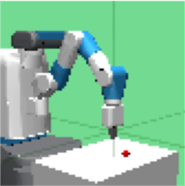
\includegraphics[height=4cm]{images/ae_input.png}};
            \node[right=.2cm of decoder] (recreated) {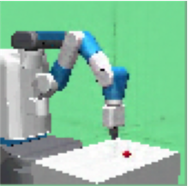
\includegraphics[height=4cm]{images/ae_recreated.png}};
            \node[below=0.5cm of original] (original_text) {Input $x$};
            \node[below=0.5cm of recreated] (recreated_text) {Reconstruction $z = f_{dec}(y)$};
            \node at (0,42 |- original_text) {$y = f_{enc}(x)$};
        \end{tikzpicture}
    \caption[High level view of an autoencoder]{High level view of an autoencoder. The reconstructed image is the actual output from an autoencoder that was trained during this work for the input image.}
    \label{fig:ae-explanation}
\end{figure}
Figure \ref{fig:ae-explanation} visualizes how an autoencoder works.

In RL, autoencoders can be used as an auxiliary loss to enhance the performance of agents trained on pixel observations. \citeauthor{yaratsImprovingSampleEfficiency2020} \cite{yaratsImprovingSampleEfficiency2020} proposed an architecture where a shared CNN feature extractor is trained by the loss of the critic and an reconstruction loss. The feature extractor is also used by the actor network, but detached during training, i.e. no updates are performed on the encoder when training the actor.

\citeauthor{kostrikovImageAugmentationAll2021} \cite{kostrikovImageAugmentationAll2021} investigated the effects of image augmentations on the performance of SAC pixels. Based on this, they developed a regularization approach called Data-regularized Q (DrQ) to enhance performance. Their idea was not simply to train the agent with augmented images but to average the Q-function over $M \geq 1$ different augmentations of the same image. Additionally, they averaged the Q target (equation \ref{eq:q-target}) over $K \geq 1$ different augmentations. A differently positioned random cropping gives the augmentations. All images from the environment have $84\times84$ pixels. First, they are padded by four pixels on each site. As padding, they used the repeated boundary pixels. Then a random crop of size $84\times84$ pixels is selected from the padded image.